\begin{document}

\def\title{Complex Numbers and Phasors}

\newcommand{\qitem}{\qpart\item}

\renewcommand{\labelenumi}{(\alph{enumi})} % change default enum format to (a)
\renewcommand{\theenumi}{(\alph{enumi})} % fix reference format accordingly.
\renewcommand{\labelenumii}{\roman{enumii}.} % second level labels.
\renewcommand{\theenumii}{\roman{enumii}.}

\maketitle

\vspace{0.5em}

% \section{Semiconductor Physics}

\qcontributor{Regina Eckert}

Generally, semiconductors are crystalline solids bonded into a lattice. In the Bohr model of the atom, the highest energy level (called the "valence" band) of an atom is considered filled when it contains 8 electrons (except the first energy level, which requires only 2 electrons). In semiconductors, atomic bonds completely "fill" the outer valence band of each atom, creating the semiconductor lattice.

	\begin{figure}[H]{
		\centering
		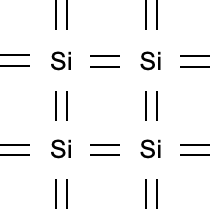
\includegraphics[width=0.2\textwidth]{n_led/si_lattice.png}
		\caption{Silicon Lattice}
		\vspace{-5mm}}
	\label{fig:SiLattice}
\end{figure}

Silicon has 4 electrons in its valence band. An electrons shared between two atoms creates a bond between those atoms. In the diagram above, a line between two silicon nuclei (designated by "Si", the symbol for silicon) represents an electron that is shared by those two silicon atoms. This electron is said to be in a "bond" between the atoms.

Sometimes, extra energy is added to the lattice. This extra energy can come from light hitting the semiconductor, like in solar cells or in digital cameras. The extra energy can also be from a voltage applied to the semiconductor, like in light-emitting diodes (LEDs). A bonded valence electron can absorb this energy. However, atomic bonds can only have a certain energy. This "excited" electron is now too energetic for the atomic bond. The excited electron can break free of the bond and move freely in the lattice. The process when light hits a semiconductor and excites an electron, breaking it free of its bond, is called the \textit{photovoltaic effect}.

When the electron breaks free of the atomic bond, it leaves a "hole" in the bond between two adjacent atoms. This hole has a positive charge because the negatively charged electron has left the bond. We can think of holes as "moving" in the semiconductor lattice, just as the electrons move. 

	\begin{figure}[H]{
		\centering
		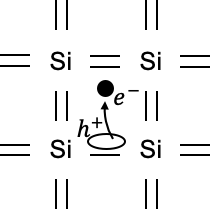
\includegraphics[width=0.2\textwidth]{n_led/si_lattice_wHole.png}
		\caption{Silicon lattice with electron $e^-$ in conduction band and hole $h^+$ where the bond is broken.}
		\vspace{-5mm}}
	\label{fig:SiLatticeWHole}
\end{figure}


Semiconductors can be visualized in terms of energy band diagrams that describe the bound ("valence band") and free ("conduction band") electrons in the semiconductor lattice. Valence band electrons have the particular energy allowed by the atomic bond, $E_V$. Conduction band electrons have minimum energy $E_C$. The energy difference between the valence and conduction bands is called the "band-gap energy", $E_G$, which is dependent on properties of the semiconductor.

	\begin{figure}[H]{
		\centering
		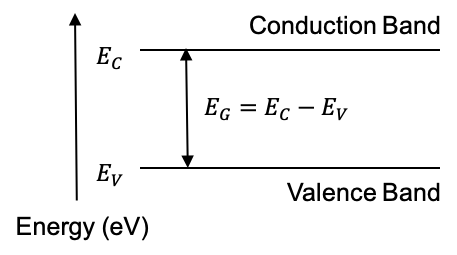
\includegraphics[width=0.4\textwidth]{n_led/band_diagram.png}
		\caption{Semiconductor energy band diagram}
		\vspace{-5mm}}
	\label{fig:BandDiagram}
\end{figure}

A conduction band electron with energy $E_C$ can recombine with a hole in the semiconductor lattice - that is, it can become a part of an atomic bond again. When this recombination happens, all of the energy that the electron has above the energy state of the valence band energy, $E_V$, gets emitted as a packet of energy. This energy can take the form of heat (a \textit{phonon}) or light (a \textit{photon}).

\subsection{Photons}
A photon is a discrete packet (or "quantum") of energy in the form of electromagnetic radiation. A photon has a particular frequency, $\nu$, of oscillation of the electromagnetic radiation. The frequency is inversely proportional to the photon's wavelength, $\lambda$. In vacuum, $\nu = \frac{c}{\lambda}$, where $c = 2.99\times10^8 m/s$ is the speed of light in a vacuum. The energy of a photon is given by $E = h\nu = \frac{hc}{\lambda}$, where $h = 4.136\times10^{-15} eV/Hz$ is Planck's constant.

Electromagnetic radiation with wavelengths between $380 ~\si{\nano\meter}$ and $700 ~\si{\nano\meter}$ (or $430-790 ~\si{\tera\hertz}$) is visible light, which can be perceived by human eyes. ($10^{12}~\si{\hertz} = 1~\si{\tera\hertz}$)

\subsection{Doping Semiconductors}

To control how current flows in a semiconductor, we have to manipulate the material's structure. We do this by "doping", or adding to, the material with other elements that have excess electrons or holes in comparison with the semiconductor.

For example, phosphorus (P) has 5 valence electrons compared to silicon's 4 valence electrons. It is added to silicon to add free electrons to the lattice, creating an "n-type" material. Similarly, we can dope semiconductors with elements that have less valence electrons than the semiconductor to make a lattice that has many holes (that is, empty electron bonds). This is called a "p-type" material. Boron (B), with 3 valence electrons, is a common p-type dopant for silicon.

It's important to note that because the elements we dope with are electrically neutral, n-type and p-type materials are also electrically neutral. That is, the material itself is not charged. This might be confusing, because we visualize n-type materials as having extra electrons and p-type materials as having extra holes, so we might think that they are negatively or positively charged. But because the number of protons and electrons is equal in a neutral element, the net charge of a doped material is still neutral. 

	\begin{figure}[H]{
		\centering
		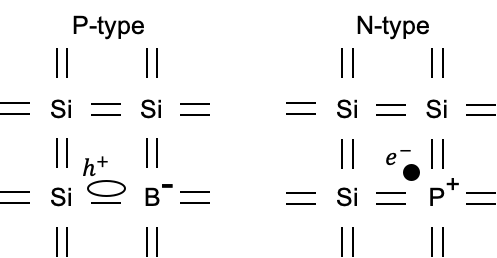
\includegraphics[width=0.4\textwidth]{n_led/doped_lattice.png}
		\caption{P-type and N-type doped lattices}
		\vspace{-5mm}}
	\label{fig:DopedSi}
\end{figure}
\iffalse
We can visualize how both holes and electrons move in the lattice in the figure below.
	\begin{figure}[H]{
		\centering
		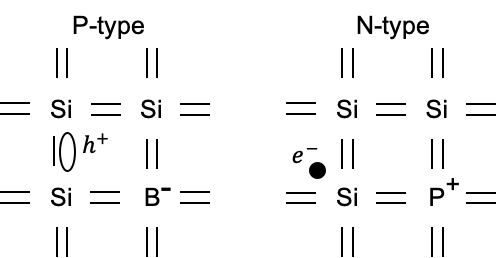
\includegraphics[width=0.4\textwidth]{n_led/doped_lattice_diffused.png}
		\caption{Movement of holes and electrons in P-type and N-type doped lattices}
		\vspace{-5mm}}
	\label{fig:DopedSi}
\end{figure}
\fi
\subsection{P-N Junction Diodes}

To create light-emitting diodes (LEDs), solar cells, and digital camera sensors, we fuse a p-type material that has a lot of extra holes in its lattice with an n-type material that has a lot of extra electrons. This is called a p-n junction diode. 

	\begin{figure}[H]{
		\centering
		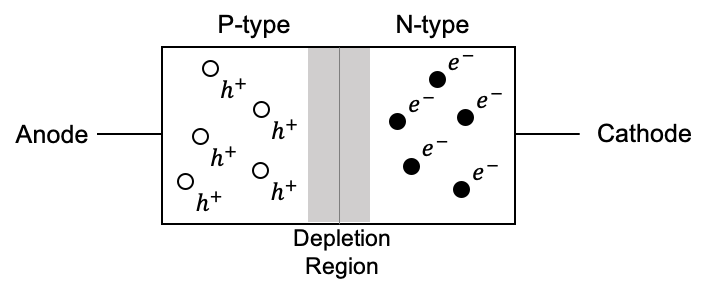
\includegraphics[width=0.5\textwidth]{n_led/pn_junction.png}
		\caption{P-N junction diode}
		\vspace{-5mm}}
	\label{fig:BandDiagramPhoton}
\end{figure}

When we first fuse the n- and p-type materials, the electrons and holes that are close to each other recombine and create a region called the "depletion region". In this region, there are no extra electrons or holes available and therefore current cannot flow across it without some help. 

When we apply a positive voltage to the p-type material (the "anode") relative to the n-type material (the "cathode"), electrons flow from the n-type to p-type material and the depletion region is decreased. This is because the electrons are attracted to the positive voltage applied at the anode and repelled by the negative voltage at the cathode. (And vice versa for the positive holes.) Current can flow across the device when this voltage is large enough that the insulating depletion region is gone. This is called a forward-bias and the diode is "on" in this case. 

However, if we apply a positive voltage to the n-type material, current does not flow. This is because the electrons are attracted to the positive voltage at the cathode, which pulls electrons out of the center of the p-n junction and increases the size of the depletion region. This means that current cannot flow across the device. In this case, the diode is "off" and no current flows from the anode to cathode.

\begin{figure}[H]{
	\centering
\begin{circuitikz} [american voltages]
	\draw
	(4,0) to[V,invert] (0,0) -- (0,2) 
	node[label={left:Anode}] {}
	to[D*,i=${I=I_d}$] (4,2)
	node[label={right:Cathode}] {}
	-- (4,0)
	;
\end{circuitikz}
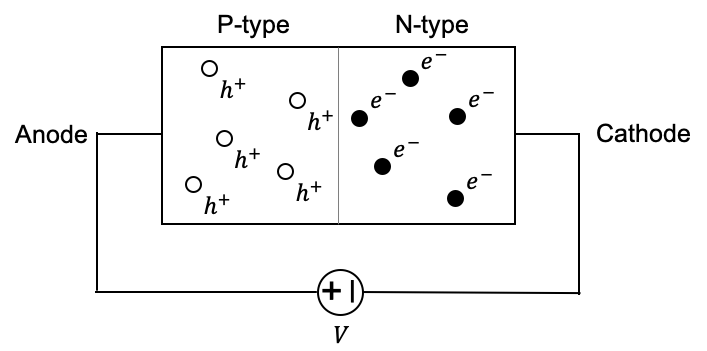
\includegraphics[width=0.4\textwidth]{n_led/pn_forward.png}
		\caption{P-N junction diode in ON state (forward-biased)}
\vspace{-5mm}}
\label{fig:pnJunctionOn}
\end{figure}

\begin{figure}[H]{
		\centering
		\begin{circuitikz} [american voltages]
			\draw
			
			(4,0) to[V] (0,0) -- (0,2) 
			node[label={left:Anode}] {}
			to[D*,i=${I=0A}$] (4,2)
			node[label={right:Cathode}] {}
			-- (4,0)
			;
		\end{circuitikz}
	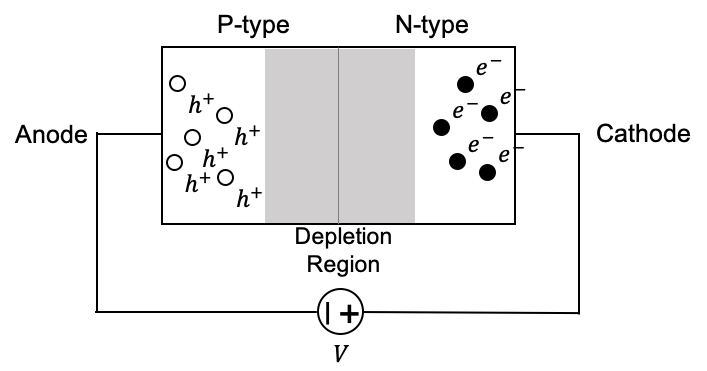
\includegraphics[width=0.4\textwidth]{n_led/pn_reverse.png}
		\caption{P-N junction diode in OFF state (reverse-biased)}
		\vspace{-5mm}}
	\label{fig:pnJunctionOff}
\end{figure}

\subsection{Light-Emitting Diodes}
LEDs are made of forward-biased p-n junction diodes. When the diode is on and current is flowing, electrons are moving across the p-n junction from the n-type through the p-type material to the anode. As they move, many electrons recombine with holes in the lattice. When this recombination happens, the electrons must emit their extra energy $E_G$ either as heat or light. LEDs are made of semiconductors that have properties such that this extra energy is more often released as light (\textit{photons}) than as heat. The photons emitted from an LED will have an energy that is equal to the band-gap energy of the semiconductor. Since a photon's energy is related to its frequency ($E=h\nu$), LED's are of specific, distinct colors determined by the semiconductor's band-gap.

Let's take a look at the energy band diagram for a recombination event. We can see that as an electron drops from the conduction band at energy $E_C$ to the valence band at energy $E_V$, it must emit energy equal to the band-gap, $E_G = E_C - E_V$. When light is emitted, $E_G$ is therefore the energy of the photon that is emitted.

	\begin{figure}[H]{
		\centering
		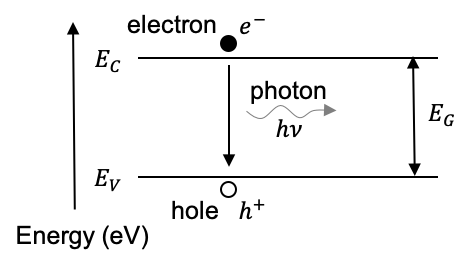
\includegraphics[width=0.4\textwidth]{n_led/band_diagram_photon.png}
		\caption{Semiconductor energy band diagram when recombination occurs and a photon is emitted}
		\vspace{-5mm}}
	\label{fig:BandDiagramPhoton}
\end{figure}

%\section{Moore's Law}

\qcontributor{Regina Eckert}

Moore's Law is a 1965 observation by Fairchild Semiconductor Research and Development Lab's director, Gordon Moore, that the number of transistors on an integrated circuit chip doubles every 1.5-2 years. This observation has dominated the computer industry into modern day, where we now have sophisticated processes to create transistors that have a smallest feature size that is 10 \si{\nano\meter} across.

\iffalse
	\begin{figure}[H]{
		\centering
		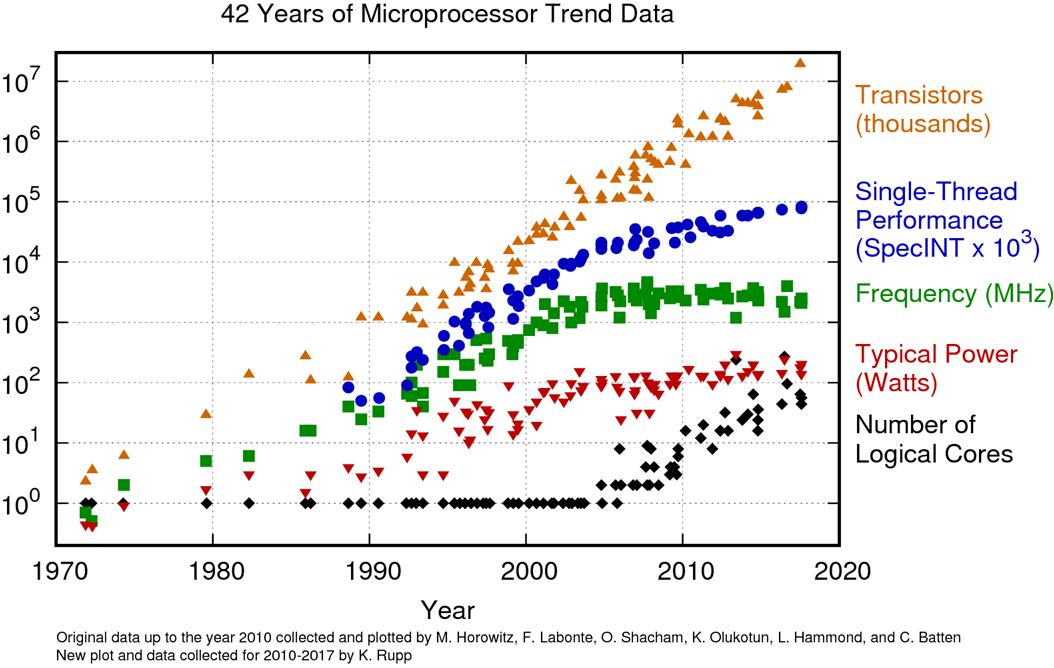
\includegraphics[width=0.8\textwidth]{n_moores_law/moores_law.png}
		\caption{Result of Moore's Law from 1970 to present day}
		\vspace{-5mm}}
	\label{fig:Moores}
\end{figure}

Figure source: https://www.karlrupp.net/.
\fi

% \newpage

\begin{qunlist}

% \qns{Design a Digital Camera Pixel}
\qcontributor{Regina Eckert}

Digital camera pixel detectors are called photodiodes. They are p-n junction diodes that use the photovoltaic effect to measure the amount of energy from light that is hitting the pixel.

\begin{enumerate}
	\qitem Should a photodiode be forward-biased (positive voltage at the anode, negative voltage at the cathode) or reverse-biased (negative voltage at the anode, positive voltage at the cathode) to generate current when a photon is absorbed? 
	
	\ans{We want to reverse-bias the photodiode. When a photon is absorbed, it creates an electron-hole pair. We want to get the electron out of the p-n junction to create current flow. 
		
	If the p-n junction is forward-biased, the negatively charged electron will be attracted to the positive voltage at the anode on the p-type side of the device. The electron will move toward the anode, but is very likely to recombine with a hole in the p-type region. In this case, the electron doesn't leave the diode and no current flows, so we cannot measure that we've collected.

However, if we reverse-bias the p-n junction, the negatively charged electron will be attracted to the positive voltage at the cathode at the n-type side of the device. Since there are very few holes in this region, the electron will not recombine inside the device. It will be able to reach the cathode, where it can be conducted away as current in the wire. Converting the photon to flowing current in the circuit means we can measure electrically how many photons have hit our photondiode!
}

	\qitem What is the minimum frequency $\nu$ that can be absorbed by a silicon photodiode? (Silicon's band-gap energy $E_G = 1.11~eV$.)
	
	\ans{The energy of a photon is $E_{photon} = h\nu$, where $h=4.136\times10^{-15} eV/Hz$ is Planck's constant. The minimum energy that can be absorbed by the solar cell is equal to the band-gap energy, $E_G$. We can therefore set the band-gap energy equal to the energy of a photon to calculate the frequency of light that is at this energy.
	
	\begin{equation}
	\nu = \frac{E_G}{h}
	\end{equation}
	
	For silicon, $E_G = 1.11~eV$, so:
	\begin{equation}
	\nu = \frac{1.11~eV}{4.136\times10^{-15} eV/Hz} = 2.684\times10^{14}~Hz = 268 ~THz.
	\end{equation}
	
	Light at this frequency is in the infrared region of the electromagnetic spectrum.
	
}
	
	\qitem If the photodiode is hit by $7\times10^{19}$ photons each second  and all of them are converted into electrons with 100\% efficiency, what is the power in Watts absorbed by the photodiode? Assume the photons are at frequency $\nu$ calculated in part (b). ($1~eV = 1.602\times10^{-19}~J$)
	
	\ans{Assuming 100\% efficiency, the energy absorbed per photon is the the photon energy, which is $E_G$ in this case.
	
	Power is given by energy/time and is in units [J/s]. To make sure our units are correct, we convert $E_G$ to units of Joules. $E_G = 1.11~eV *\frac{1.602\times10^{-19}~J}{1~eV} = 1.7782 \times 10^{-19}~J$.
	
	To calculate the power absorbed, we must multiply the energy per photon by the rate that photons hit the photodiode:
	\begin{equation}
	P = E_G * rate_{photon} = (1.7782 \times 10^{-19}~J/photon)*(7\times 10^{19}~photons/s)= 12.45 W
	\end{equation}
}

	\qitem Irradiance is the power received per unit area and has units $[W/m^2]$. If the photodiode's area $A_{diode} = 0.1~m^2$, what is the irradiance incident on the photodiode for photons at frequency $\nu$ at a $rate_{photon} = 7\times10^{19}$ photons/second?
	
	\ans{ From the description, we can write the irradiance $Irr$ as:
		
		\begin{equation}
		Irr = \frac{P}{A_{diode}}.
		\end{equation} 
		
		Using the power calculated in part (c),
		
		\begin{equation}
		Irr = \frac{E_G * rate_{photon}}{A_{diode}}=(1.7782 \times 10^{-19}~J/photon)*(7\times 10^{19}~photons/s)/0.1~m^2 = 124.5 W/m^2
		\end{equation} 
	}
	
	\iffalse
	\qitem If we apply a voltage $V = 10V$ across the solar cell p-n junction to bias it, and it is generating the power $P$ we calculated in (c), what current $I$ is flowing from the solar cell?
	
	\ans{We know that $P=IV$. Therefore, $I = P/V$. Plugging in with the power from part (c), we find:
	
	\begin{equation}
	I = \frac{12.45~W}{10V} = 1.245~A.
	\end{equation}

}
	
	\qitem Since the solar cell has a voltage $V$ across it and a current $I$ through it, we might think of modeling it as a resistive load. What resistance $R$ would this solar cell have if $V = 10V$?
	
	\ans{ We know that $V = IR$, or $R = V/I$. Plugging in the current from part (e), we find:
	\begin{equation}
	R = \frac{10~V}{1.245~A} = 8.03 \si{\ohm}
	\end{equation}
}
\fi
	
\end{enumerate}	
% {\Large \textbf{Mechanical:}}
\qns{First-Order Differential Equation Practice}


\begin{enumerate}

\qitem Solve the equation $\frac{d}{dt} f(t) = 7 f(t) $ given that $f(0) = 3$

\sol{
	$f(t) = 3 e^{7t}$.
}

\qitem Solve the equation $\frac{d}{dt} f(t) + 5 f(t) = 0 $ given that $f(0) = 2$

\sol{
	$f(t) = 2 e^{-5t}$.
}

\qitem Solve the equation $3 \frac{d}{dt} f(t) + 6 f(t) = 0$ given that $f(0) = 7$

\sol{

	% We know that the solution to the first-order differential equation must be of the form $f(t) = A e^{\lambda t} + B$. If we plug in that definition of $f(t)$ into the given equation, we get
	% \begin{align*}
	% 	3 (A \lambda e^{\lambda t}) + 6(A e^{\lambda t} + B) &= 0 \\
	% 	(3 A \lambda + 6 A)e^{\lambda t} + 6B &= 0
	% \end{align*}
	% We know that the coefficient of the exponential $e^{\lambda t}$ and the constant must be zero, which means that $3A \lambda + 6A = 0$ and $6B = 0$. Solving these yield $\lambda = -2, B = 0$. If we use our initial condition alongside the parameters we just found, we get $7 = f(0) = A e^{-2 (0)} + 0 = A$, implying that $A = 7$. Therefore, 
	$f(t) = 7 e^{-2t}$.
	
}

\qitem Solve the equation $\frac{d}{dt} f(t) = 2f(t) + 2 $ given that $f(0) = 3$

\sol{
	$f(t) = 4 e^{2t} - 1$.
}


\qitem Solve the equation $5\frac{d}{dt} f(t) + 3f(t) - 10 = 0 $ given that $f(0) = 8$

\sol{
	$f(t) = \frac{14}{3}e^{\frac{-3}{5} t} + \frac{10}{3}$.
}



\qitem Solve the equation $6\frac{d}{dt} f(t) + 4 = 3f(t) $ given that $f(0) = \frac{1}{3}$

\sol{
	$f(t) = - e^{\frac{1}{2} t} + \frac{4}{3} $.
}


\qitem Solve the equation $3f(t) - 6 f'(t) = 4$ given that $f(2) = \frac{1}{3}$

\sol{
	% $f(t) = A e^{\lambda t} + B$
	% \begin{align*}
	% 	3 (A e^{\lambda t} + B) - 6(A \lambda e^{\lambda t}) &= 4 \\
	% 	(3A - 6A \lambda) e^{\lambda t} + 3B &= 4 \\
	% 	\lambda &= \frac{1}{2} \\
	% 	B &= \frac{4}{3} \\
	% 	f(t) &= A e^{\frac{1}{2} t} + \frac{4}{3} \\
	% 	f(2) = \frac{1}{3} &= A e^{\frac{1}{2}(2)} + \frac{4}{3} \\
	% 	A &= -\frac{1}{e} \\
	% 	f(t) &= -\frac{1}{e} e^{\frac{1}{2} t} + \frac{4}{3} \\
	% 	&= -e^{\frac{1}{2} t - 1} + \frac{4}{3} \\
	% \end{align*}
	$f(t) = -e^{\frac{1}{2} t - 1} + \frac{4}{3}$ \\
	
}

% \qitem  Solve the equation $f'(t) = 5f(t) + 8 e^{5t}$ given that $f(0) = 7$

% \sol{
% 	$7e^{5t}+8e^{5t}t$.
% }


% \qitem  Solve the equation $f'(t) = af(t) + k e^{bt}$

% \sol{
% 	$ce^{at}-\frac{ke^{bt}}{a-b}$.
% }



\end{enumerate}
\input{mech2}
\input{q1}
\input{q2}	
% \qns{Phasor-domain circuit analysis}
\qcontributor{Yuxun Zhou}

The analysis techniques you learned previously for resistive circuits
are equally applicable for analyzing AC circuits (circuits driven by
sinusoidal inputs) in the phasor domain. In this problem, we will walk
you through the steps with a  concrete example. Consider the circuit
below. 

	\begin{center}
		\begin{circuitikz}[scale=0.8]
			\draw node[ground] {} (0,0)	
			to[short] (5,0)
			(5,2) to[V = $v(t)$] (5,0)
			(5,2) to[R = $R_2$,i<=$i_{R2}$] (5,4)
			to[short] (5,6)
			to[R = $R_1$,i=$i_{R1}$] (0,6)
			to[short] (0,3)
			to[C = $C_1$] (0,2)
			to[short,i = $i_c$] (0,1.5)
			to[short] (0,0);			
		
			\draw (0,4)
			to[L = $L_1$,i<=$i_{L1}$, *-*] (5,4)
			to[L = $L_2$,i=$i_{L2}$] (10,4)
			to[R = $R_3$] (10,0)
			to[short] (5,0);
			
			\draw (0,4) node[label={left:$N_1$}] {}	;
			\draw (5,4) node[label={45:$N_2$}] {}	;

		\end{circuitikz}
	\end{center}

The components in this circuit are given by:

Voltage source:
$$v(t) = 20\cos (50t-\frac{\pi}{3})$$ 
Resistors:
$$R_1 = 8\Omega,\quad R_2 = 8\Omega, \quad R_3 = 8\Omega$$
Inductors: 
$$L_1 = 40 \; \text{mH},\quad L_2 = 40 \; \text{mH}$$
Capacitor:
$$C_1 = 5 \;\text{mF}$$

\begin{enumerate}

\qitem To begin with, transform the given circuit to the phasor domain. 

\sol{
\begin{align*}
Z_L &= j\omega L = j50\times 40 \times 10^{-3} = j2\; \Omega \\
Z_C &= \frac{1}{j\omega C} =\frac{1}{j50\times 5 \times 10^{-3}}= -j4\; \Omega \\
\widetilde{v} &=|v|e^{j\angle v} = 20e^{-j\frac{\pi}{3}}
\end{align*}
 }

\qitem Write out KCL for node $N_1$ and $N_2$ in the phasor domain.

\sol{
\begin{align*}
\intertext{At node 1}
i_{L1}+i_{R1} &= i_c \\
\intertext{At node 2}
i_{R1}+i_{L1}+i_{R2}+i_{L2}&=0 \\
\end{align*}
}

\qitem Use KVL to express the currents in terms of node voltages in the phasor domain. The node voltages $\widetilde{V}_1$ and $\widetilde{V}_2$ are the voltage drops from $N_1$ and $N_2$ to the ground.

\sol{We have
\begin{align*}
\frac{\widetilde{V}_2-\widetilde{V}_1}{Z_L} + \frac{\widetilde{V}_2-\widetilde{V}_1}{R}  &=\frac{\widetilde{V}_1}{Z_C}   \\
\frac{\widetilde{V}_2-\widetilde{V}_1}{R} + \frac{\widetilde{V}_2-\widetilde{V}_1}{Z_L} + \frac{\widetilde{V}_2-\widetilde{v}}{R} + \frac{\widetilde{V}_2}{R+Z_L}&=0 
\intertext{Plugging in values from part (a), we get}
\frac{\widetilde{V}_2-\widetilde{V}_1}{j2} + \frac{\widetilde{V}_2-\widetilde{V}_1}{8}  &=\frac{\widetilde{V}_1}{-j4}  \\
\frac{\widetilde{V}_2-\widetilde{V}_1}{8} + \frac{\widetilde{V}_2-\widetilde{V}_1}{j2} + \frac{\widetilde{V}_2-20e^{-j\frac{\pi}{3}}}{8} + \frac{\widetilde{V}_2}{8+j2}&=0
\intertext{For future parts, we want the denominators of each current to be either purely real or purely imaginary. To put $i_{L2}$ in this form, we can manipulate the expression by multiplying the denominator by its conjugate:}
\frac{\widetilde{V}_2}{8+j2}\bigg(\frac{8-j2}{8-j2}\bigg)=\frac{\widetilde{V}_2(8-j2)}{8^2-(-4)} &= \frac{\widetilde{V}_2(8-j2)}{68} 
\intertext{Our final KCL equations at nodes $N_1$ and $N_2$ are}
\frac{\widetilde{V}_2-\widetilde{V}_1}{j2} + \frac{\widetilde{V}_2-\widetilde{V}_1}{8}  &=\frac{\widetilde{V}_1}{-j4}  \\
\frac{\widetilde{V}_2-\widetilde{V}_1}{8} + \frac{\widetilde{V}_2-\widetilde{V}_1}{j2} + \frac{\widetilde{V}_2-20e^{-j\frac{\pi}{3}}}{8} + \frac{\widetilde{V}_2(8-j2)}{68}&=0
\end{align*}
}

\qitem Write the equations you derived in part (b) and (c) in a matrix form, i.e., $A\begin{bmatrix}
\widetilde{V}_1\\\widetilde{V}_2
\end{bmatrix} = b$ Solve for $A$ and $b$ in numerical form.

\sol{ From the above two equations, we have
\begin{align*}
 A = \begin{bmatrix}
\frac{1}{8} - j\frac{1}{4} & -\frac{1}{8} + j\frac{1}{2} \\
-\frac{1}{8} + j\frac{1}{2} & \frac{1}{4} + \frac{8}{68} - j\frac{1}{2} - j\frac{2}{68}
\end{bmatrix} &= 
\begin{bmatrix}
   0.125 - j0.25 & -0.125 + j0.5\\
  -0.125 + j0.5 & 0.3676 + j0.5294
\end{bmatrix} \\
b = \begin{bmatrix}
0\\ \frac{20e^{-j\frac{\pi}{3}}}{8}
\end{bmatrix} &= 
\begin{bmatrix}
0\\ 1.25 - j2.165
\end{bmatrix}
\end{align*}
 }

\qitem Solve the systems of linear equations you derived in part (d) with any method you prefer, and then find $i_c(t)$.

\sol{ 2 by 2 matrix is easy to be inverted, .i.e.,
$$
\begin{bmatrix}
a & b\\ c &d
\end{bmatrix}^{-1}
= \frac{1}{ad-bc}  \begin{bmatrix}
d & -b \\ -c & a
\end{bmatrix} $$
$$
A^{-1} =
\begin{bmatrix}
  3.1280 - j2.8782 &  1.5240 - j3.0381 \\
  1.5240 - j3.0381 &  1.1643 - j1.4291
\end{bmatrix} \\
$$

With that we find
$$
\begin{bmatrix}
\widetilde{V}_1\\ \widetilde{V}_2
\end{bmatrix} = A^{-1} b =
\begin{bmatrix}
-4.6726 - j7.0973 \\ -1.6388 - j4.3071
\end{bmatrix}
=\begin{bmatrix}
8.4973e^{-j2.1530}\\4.6083e^{-j1.9344}
\end{bmatrix}
$$
Then $$I_C = \frac{\widetilde{V}_1}{-j4} = \frac{j}{4} \widetilde{V}_1 = 2.1243e^{-j0.5822}$$
transform back to time domain we have
$$i_C(t) = 2.1243\cos (50t-0.5822)$$
}


\end{enumerate}

\begin{comment}
Other analysis techniques?
\end{comment}

% q3 uses the phasor definition from previous iterations of 16B.
\input{q4}	

\end{qunlist}

\end{document}
